%%%%%%%%%%%%%%%%%%%%%%%%%%%%%%%%%%%%%%%%%%%%%%%%%%%%%%%%%%%%%%%%%%%%%%
% Problem statement
\begin{statement}[
  problempoints=110,
  timelimit=1 sekunda,
  memorylimit=512 MiB,
]{Konstrukcija}

%\setlength\intextsep{-0.1cm}
%\begin{wrapfigure}[7]{r}{0.27\textwidth}
%\centering
%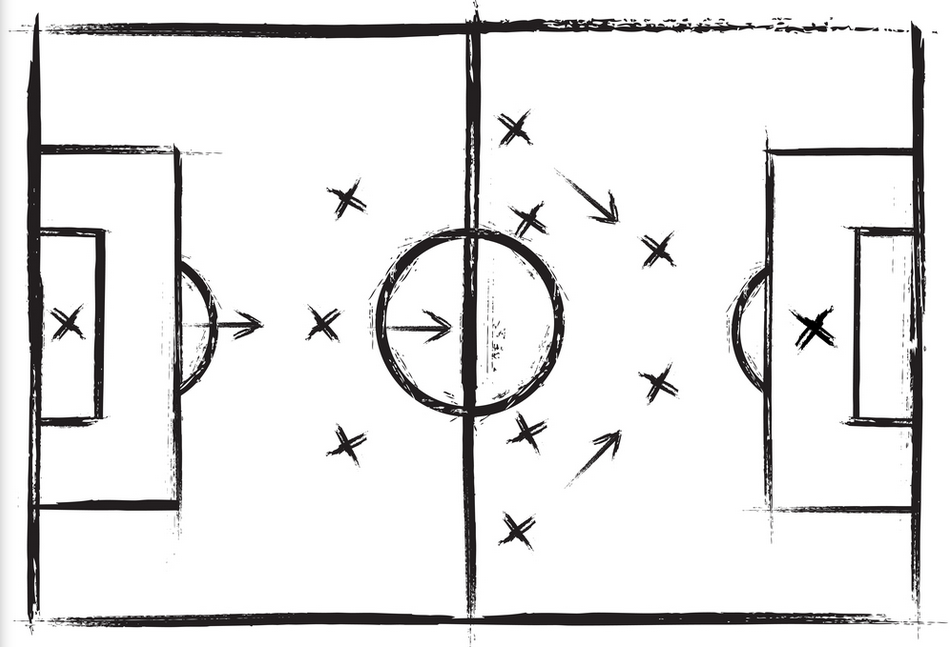
\includegraphics[width=0.27\textwidth]{img/trener.png}
%\end{wrapfigure}


Let $G$ be a directed acyclic graph. If $c_1, c_2, c_3, \dots c_n$ are distinct
vertices of $G$ such that there is a path from $c_1$ to $c_2$, there is a
path from $c_2$ to $c_3$, \dots and there is a path from $c_{n-1}$ to $c_n$,
we say that array $C = (c_1, c_2, c_3, \dots c_n)$ is an ordered array
starting at $c_1$ and ending at $c_n$. Note that between neighbouring
elements $c_i$ and $c_{i+1}$ of ordered array $C$ it isn't necessary to exist
a direct edge, it is enough for the path to exist from $c_i$ to $c_{i+1}$.

For this definition of an ordered array $C = (c_1, c_2, c_3, \dots c_n)$, we
define its length $len(C) = n$.  Therefore, the length of an ordered array
is equal to the number of vertices it holds. Note that the ordered array
can have a length of $1$ when holding a single vertex which represents both
its beginning and its end.

Also, for an ordered array $C = (c_1, c_2, c_3, \dots c_n)$ we can define its
sign as $sgn(C) = (-1)^{len(C)+1}$.  For vertices $x$ and $y$ of
$G$, let's denote with $S_{x,y}$ a set of all ordered arrays that start in $x$
and end in $y$.

Finally, we define the tension between nodes $x$ and $y$ as $tns(x, y)=\sum_{C \in
S_{x, y}}{sgn(C)}$. Therefore, the tension between nodes $x$ and $y$ equals the
sum of signs of all ordered arrays that start in $x$ and end in $y$.

An integer $K$ is given. Your task is to construct a directed acyclic graph
with \textbf{at most 1000} vertices and \textbf{at most 1000} edges for
which $tns(1, N) = K$ holds. Number $N$ in the previous expression denotes
the number of vertices in a graph. Vertices of a graph should be indexed
using positive integers from $1$ to $N$.

%%%%%%%%%%%%%%%%%%%%%%%%%%%%%%%%%%%%%%%%%%%%%%%%%%%%%%%%%%%%%%%%%%%%%%
% Input
\subsection*{Input}
The first line contains an integer $K$ $(|K| \le 10^{18})$ from the
task description.

%%%%%%%%%%%%%%%%%%%%%%%%%%%%%%%%%%%%%%%%%%%%%%%%%%%%%%%%%%%%%%%%%%%%%%
% Output
\subsection*{Output}
In the first line you should output the number of vertices and the number of
edges of the constructed graph. Let's denote the number of vertices of that
graph with $N$ $(1 \le N \le 1000)$, and the number of edges with $M$ $(0 \le
M \le 1000)$.

In the $i$-th of the next $M$ lines you should output two distinct integers
$X_i$ and $Y_i$ $(1 \le X_i, Y_i \le N)$, which represent the $i$-th edge which
is directed from vertex with index $X_i$ towards vertex with index $Y_i$. Each
edge must appear only once in the output.

Also, the absolute value of tension between each two nodes in the graph must
be less or equal to $2^{80}$.

If there are multiple solutions, output any of them.

%%%%%%%%%%%%%%%%%%%%%%%%%%%%%%%%%%%%%%%%%%%%%%%%%%%%%%%%%%%%%%%%%%%%%%
% Scoring
\subsection*{Scoring}
{\renewcommand{\arraystretch}{1.4}
  \setlength{\tabcolsep}{6pt}
  \begin{tabular}{ccl}
 Subtask & Score & Constraints \\ \midrule
  1 & 15 & $1 \le K < 500$ \\
  2 & 15 & $-300 < K \le 1$ \\
  3 & 20 & $|K| < 10000$\\
  4 & 60 & No additional constraints. \\
\end{tabular}}

%%%%%%%%%%%%%%%%%%%%%%%%%%%%%%%%%%%%%%%%%%%%%%%%%%%%%%%%%%%%%%%%%%%%%%
% Examples
\subsection*{Examples}
\begin{tabularx}{\textwidth}{X'X'X}
\sampleinputs{test/konstrukcija.dummy.in.1}{test/konstrukcija.dummy.out.1} &
\sampleinputs{test/konstrukcija.dummy.in.2}{test/konstrukcija.dummy.out.2} &
\sampleinputs{test/konstrukcija.dummy.in.3}{test/konstrukcija.dummy.out.3}
\end{tabularx}

\textbf{Clarification of the first example:}
The constructed graph has $6$ vertices. Ordered arrays that start in $1$ and
end in $6$ are: $(1, 6)$, $(1, 4, 6)$, $(1, 5, 6)$, $(1, 3, 6)$, $(1, 2, 6)$,
$(1, 4, 3, 6)$, $(1, 4, 2, 6)$, $(1, 5, 3, 6)$, $(1, 5, 2, 6)$, $(1, 3, 2, 6)$,
$(1, 4, 3, 2, 6)$, $(1, 5, 3, 2, 6)$. Their lengths are (in order): $1, 2, 2,
2, 2, 3, 3, 3, 3, 3, 4, 4$, so their signs are $-1, 1, 1, 1, 1, -1, -1, -1, -1,
-1, 1, 1$. Therefore, the tension between $1$ and $6$ is equal to $-1 + 1 + 1 +
1 + 1 - 1 - 1 - 1 - 1 - 1 + 1 + 1 = 0$.

\setlength\intextsep{-0.5cm}
\begin{wrapfigure}{c}{\textwidth}
\centering
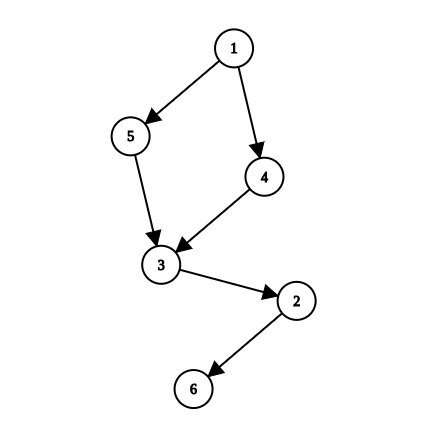
\includegraphics[width=0.6\textwidth]{graph.png}
\end{wrapfigure}

%%%%%%%%%%%%%%%%%%%%%%%%%%%%%%%%%%%%%%%%%%%%%%%%%%%%%%%%%%%%%%%%%%%%%%
% We're done
\end{statement}

%%% Local Variables:
%%% mode: latex
%%% mode: flyspell
%%% ispell-local-dictionary: "croatian"
%%% TeX-master: "../hio.tex"
%%% End:
